\chapter{Architecture et Conception du Système}
\label{chap:architecture_conception}

\section*{Introduction}
\addcontentsline{toc}{section}{Introduction}
Suite à l'analyse détaillée des besoins, ce chapitre est consacré à la conception technique de la solution. Nous y présenterons l'architecture globale de l'application, les choix technologiques adoptés, ainsi que la modélisation statique (diagramme de classes) et dynamique (diagrammes de séquence) du système. Enfin, nous détaillerons les mécanismes de sécurité mis en place pour garantir l'intégrité des données industrielles.

% ---------------------------------------------------------
\section{Architecture Globale et Choix Technologiques}

\subsection{Pattern d'Architecture}
L'application repose sur une architecture découplée de type \textbf{Client/Serveur} (Single Page Application + API REST).
Le backend adopte une architecture en couches inspirée du \textbf{Domain-Driven Design (DDD)}, séparant strictement la logique de présentation (API/Routes), la logique métier (Services) et l'accès aux données (Modèles). Le frontend, quant à lui, est structuré par fonctionnalités (\textit{Feature-Driven Component-Based}).

\begin{figure}[H]
    \centering
    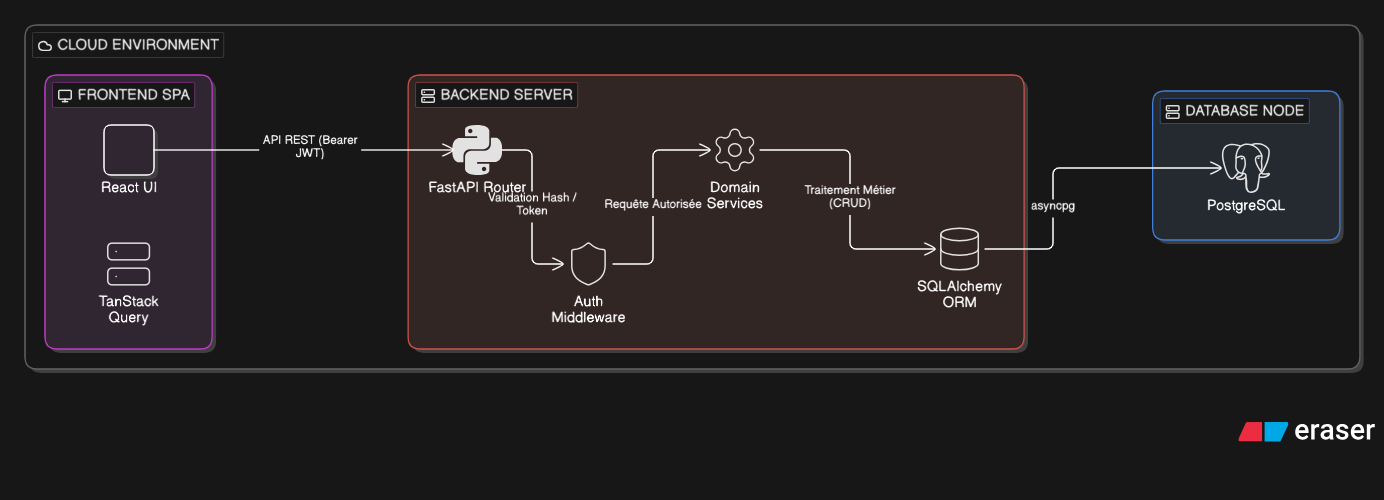
\includegraphics[width=0.8\textwidth]{images/ch4/arch.png}
    \caption{Architecture globale et flux de communication du système}
    \label{fig:architecture_globale}
\end{figure}

\subsection{Stack Technologique}
Pour répondre aux exigences de performance et de modernité, les technologies suivantes ont été retenues :

\begin{itemize}
    \item \textbf{Frontend (Client Web) :} 
    \begin{itemize}
        \item \textbf{React 19 (TypeScript) / Vite :} Pour un typage statique strict et un rendu réactif.
        \item \textbf{Tailwind CSS v4 :} Pour un design système rapide et responsive.
        \item \textbf{TanStack Query :} Pour la mise en cache intelligente et la gestion asynchrone des requêtes.
        \item \textbf{Chart.js :} Pour la visualisation dynamique des tendances des KPIs.
    \end{itemize}
    
    \item \textbf{Backend (API REST) :}
    \begin{itemize}
        \item \textbf{Python (FastAPI) :} Choisi pour ses hautes performances (asynchrone natif) et sa génération automatique de documentation (Swagger/OpenAPI).
        \item \textbf{SQLAlchemy 2.0 \& Pydantic v2 :} Pour le mapping objet-relationnel (ORM) asynchrone et la validation stricte des flux d'entrée/sortie.
    \end{itemize}
    
    \item \textbf{Base de données :} 
    \begin{itemize}
        \item \textbf{PostgreSQL :} Déployé via le driver asynchrone \texttt{asyncpg}, garantissant robustesse et intégrité relationnelle.
    \end{itemize}
\end{itemize}

\subsection{Étude Comparative et Justification des Choix (Benchmark)}
Le choix d'une architecture découplée \textbf{FastAPI (Backend) + React SPA (Frontend)} face à un framework full-stack unifié tel que \textbf{Next.js} (Node.js) a été guidé par les contraintes spécifiques du contexte industriel de SEBN-MA. Le tableau~\ref{tab:benchmark_archi} résume cette analyse comparative.

\begin{table}[H]
\centering
\small
\renewcommand{\arraystretch}{1.3}
\begin{tabular}{|p{3.8cm}|p{5.5cm}|p{5.5cm}|}
\hline
\textbf{Critère d'évaluation} & \textbf{Next.js (Monolithe Full-Stack Node.js)} & \textbf{Solution Retenue : FastAPI + React SPA} \\
\hline
\hline
\textbf{Nature de l'application \& Référencement (SEO)} & Conçu pour le rendu côté serveur (SSR) et le SEO public (e-commerce, vitrines). & Application intranet métier dédiée. Le SSR est inutile ; une SPA client-side servie statiquement offre une fluidité maximale. \\
\hline
\textbf{Écosystème Data \& Calculs Industriels} & Écosystème JavaScript limité pour l'analyse mathématique et statistique avancée. & Écosystème Python incontournable (NumPy, Pandas, SciPy), ouvrant la voie à la maintenance prédictive et au Machine Learning. \\
\hline
\textbf{Interopérabilité \& API First} & Logique serveur souvent couplée aux Server Actions et composants React. & API REST pure, documentée nativement (\textit{OpenAPI/Swagger}), facilement consommable par des scripts Python et macros Excel. \\
\hline
\textbf{Performances d'ingestion (I/O intensives)} & Bonnes performances en I/O, mais ORMs Node.js (ex: Prisma) plus lourds en écriture de masse. & Moteur asynchrone (\textit{Starlette + Pydantic v2} en Rust) avec driver \texttt{asyncpg}, offrant un débit exceptionnel en \textit{Bulk Insert}. \\
\hline
\textbf{Déploiement en milieu industriel (On-Premise)} & Nécessite un runtime Node.js permanent ou des fonctions Serverless (ex: Vercel). & Découplage total : API conteneurisée (Docker léger) et Frontend compilable en fichiers statiques (Nginx/CDN). \\
\hline
\end{tabular}
\caption{Comparatif architectural : Next.js versus FastAPI / React SPA}
\label{tab:benchmark_archi}
\end{table}

Cette analyse met en lumière trois arguments décisifs en faveur de la solution retenue :
\begin{enumerate}
    \item \textbf{La vocation multi-clients de l'API (Approche API-First) :} L'application ne s'adresse pas uniquement aux navigateurs web. La phase 2 du projet requiert l'ingestion automatique de données issues de macros Excel et de scripts d'automatisation. FastAPI permet d'exposer une API REST découplée, standardisée, validée par Pydantic et sécurisée par clés d'API, indépendamment du cycle de vie de l'interface graphique.
    \item \textbf{La synergie avec le traitement de données industrielles :} Python constitue la référence absolue pour le traitement des séries temporelles et le calcul des métriques de production (OEE, Scrap Rate, CIM). L'utilisation de FastAPI garantit une intégration naturelle avec les futures briques d'intelligence artificielle et d'analyse prédictive envisagées par l'usine.
    \item \textbf{L'absence de besoin en rendu serveur (SSR) :} Les tableaux de bord de supervision interne ne nécessitent aucun référencement naturel. L'utilisation d'une Single Page Application (SPA) propulsée par React 19 et \textit{TanStack Query} élimine la charge serveur liée au SSR, tout en assurant une mise en cache locale instantanée pour les utilisateurs sur les lignes de production.
\end{enumerate}

% ---------------------------------------------------------
\section{Modélisation de la Base de Données}
La structuration des données est le cœur de notre application. Elle doit permettre de relier efficacement les équipements (machines HCM-S et CIM-3) à leurs indicateurs de performance, tout en conservant une traçabilité totale.

\begin{figure}[H]
    \centering
    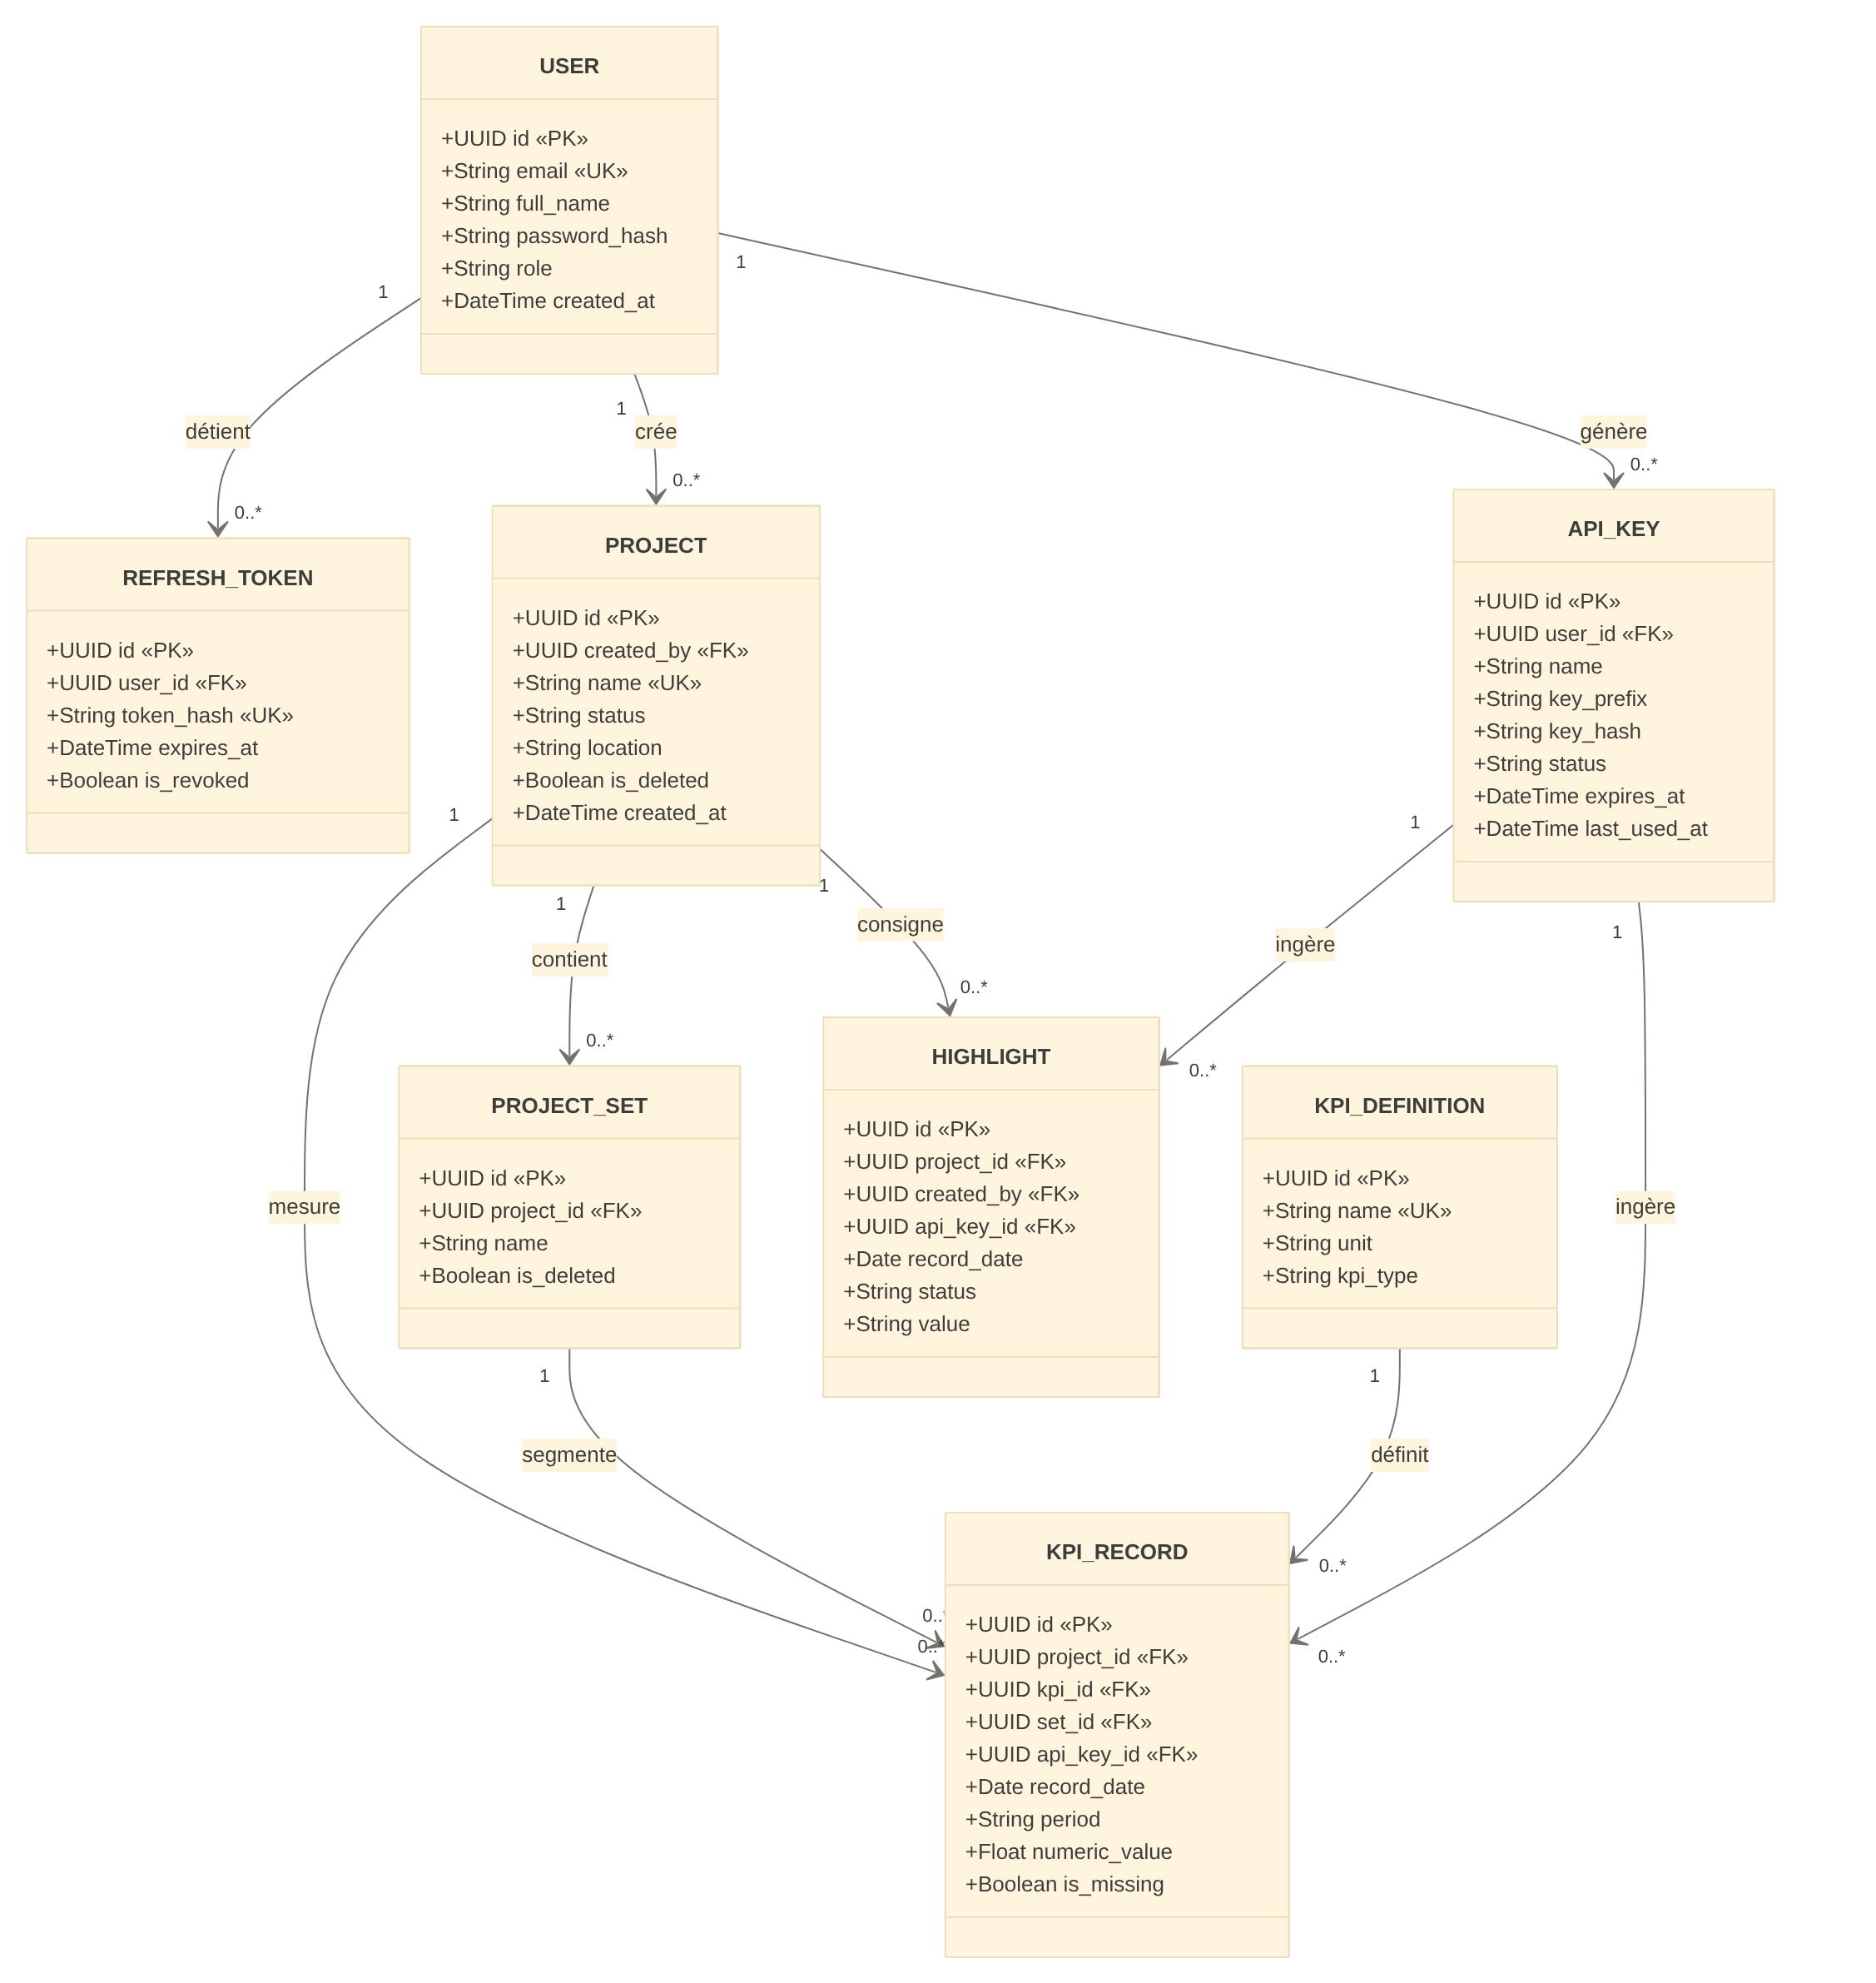
\includegraphics[width=0.9\textwidth]{images/ch4/uml_class.png}
    \caption{Diagramme de classes UML}
    \label{fig:diagramme_classes}
\end{figure}

\subsection{Entités Principales}
Le modèle relationnel s'articule autour de deux axes majeurs :
\begin{enumerate}
    \item \textbf{Axe Structurel et Sécurité :}
    \begin{itemize}
        \item \textbf{User :} Gère les administrateurs avec leurs rôles (Admin, Super Admin).
        \item \textbf{ApiKey :} Stocke les clés d'ingestion automatisées pour la Phase 2.
    \end{itemize}
    \item \textbf{Axe Métier (Industriel) :}
    \begin{itemize}
        \item \textbf{Project \& ProjectSet :} Représentent les lignes de production et leurs sous-ensembles machines (le "Set" HCM-S / CIM-3).
        \item \textbf{KPIDefinition :} Le référentiel des métriques mesurées (ex: TRS, Absentéisme, Qualité) avec leurs unités.
        \item \textbf{KPIRecord \& Highlight :} Les valeurs réelles mesurées dans le temps et les faits marquants associés.
    \end{itemize}
\end{enumerate}

\subsection{Stratégie de "Soft Delete" et Intégrité}
Dans un contexte industriel, la perte de données statistiques est inacceptable. C'est pourquoi une stratégie de suppression logique (\textit{Soft Delete}) a été implémentée :
\begin{itemize}
    \item \textbf{Drapeau Booléen :} Les projets et sets de machines ne sont jamais détruits physiquement de la base. Un attribut \texttt{is\_deleted = True} les masque des requêtes courantes, préservant ainsi l'historique des KPIs associés.
    \item \textbf{Machine à états pour les clés API :} Une clé passe de \textit{ACTIVE} à \textit{REVOKED} puis \textit{DELETED}. La clé est conservée pour garantir l'auditabilité des enregistrements (\texttt{api\_key\_id}) ayant été ingérés dans le passé.
\end{itemize}

% ---------------------------------------------------------
\section{Sécurité et Gestion des Accès}
La plateforme HCM-S CIM3 expose des données sensibles et nécessite une gestion stricte des identités, répartie en trois niveaux (Visiteur, Admin, Super Admin).

\subsection{Authentification des utilisateurs (JWT)}
Les accès humains sont gérés via le standard JSON Web Token (JWT) avec un motif à double jeton (\textit{Double Token Pattern}) :
\begin{itemize}
    \item Un \textbf{Access Token} de courte durée (utilisé pour les requêtes API).
    \item Un \textbf{Refresh Token} de longue durée, stocké sous forme de condensat (hash) en base, permettant de renouveler la session de manière transparente grâce à des intercepteurs \texttt{Axios} côté Frontend.
\end{itemize}

\subsection{Sécurisation de l'Ingestion (API Keys)}
Pour la Phase 2 (l'automatisation par script), l'authentification s'effectue via des clés d'API. Le backend applique le principe de \textit{Zero-Knowledge Storage} :
La clé générée n'est affichée qu'une seule fois à l'utilisateur. Seul un condensat cryptographique fort (\textbf{SHA-256}) est stocké en base de données. Lors d'une requête, le backend recalcule le hash du jeton reçu et le compare à celui stocké, garantissant qu'une compromission de la base de données ne révèle pas les clés d'accès.

% ---------------------------------------------------------
\section{Conception Dynamique : Diagrammes de Séquence}
Pour illustrer le comportement dynamique du système, nous avons modélisé les deux processus critiques du cycle de vie de la donnée : son ingestion et sa restitution.

\subsection{Phase 1 : Ingestion Automatisée des KPIs}
Le flux suivant décrit l'action du script externe poussant les données de la Macro Excel vers l'API.

\begin{figure}[H]
    \centering
    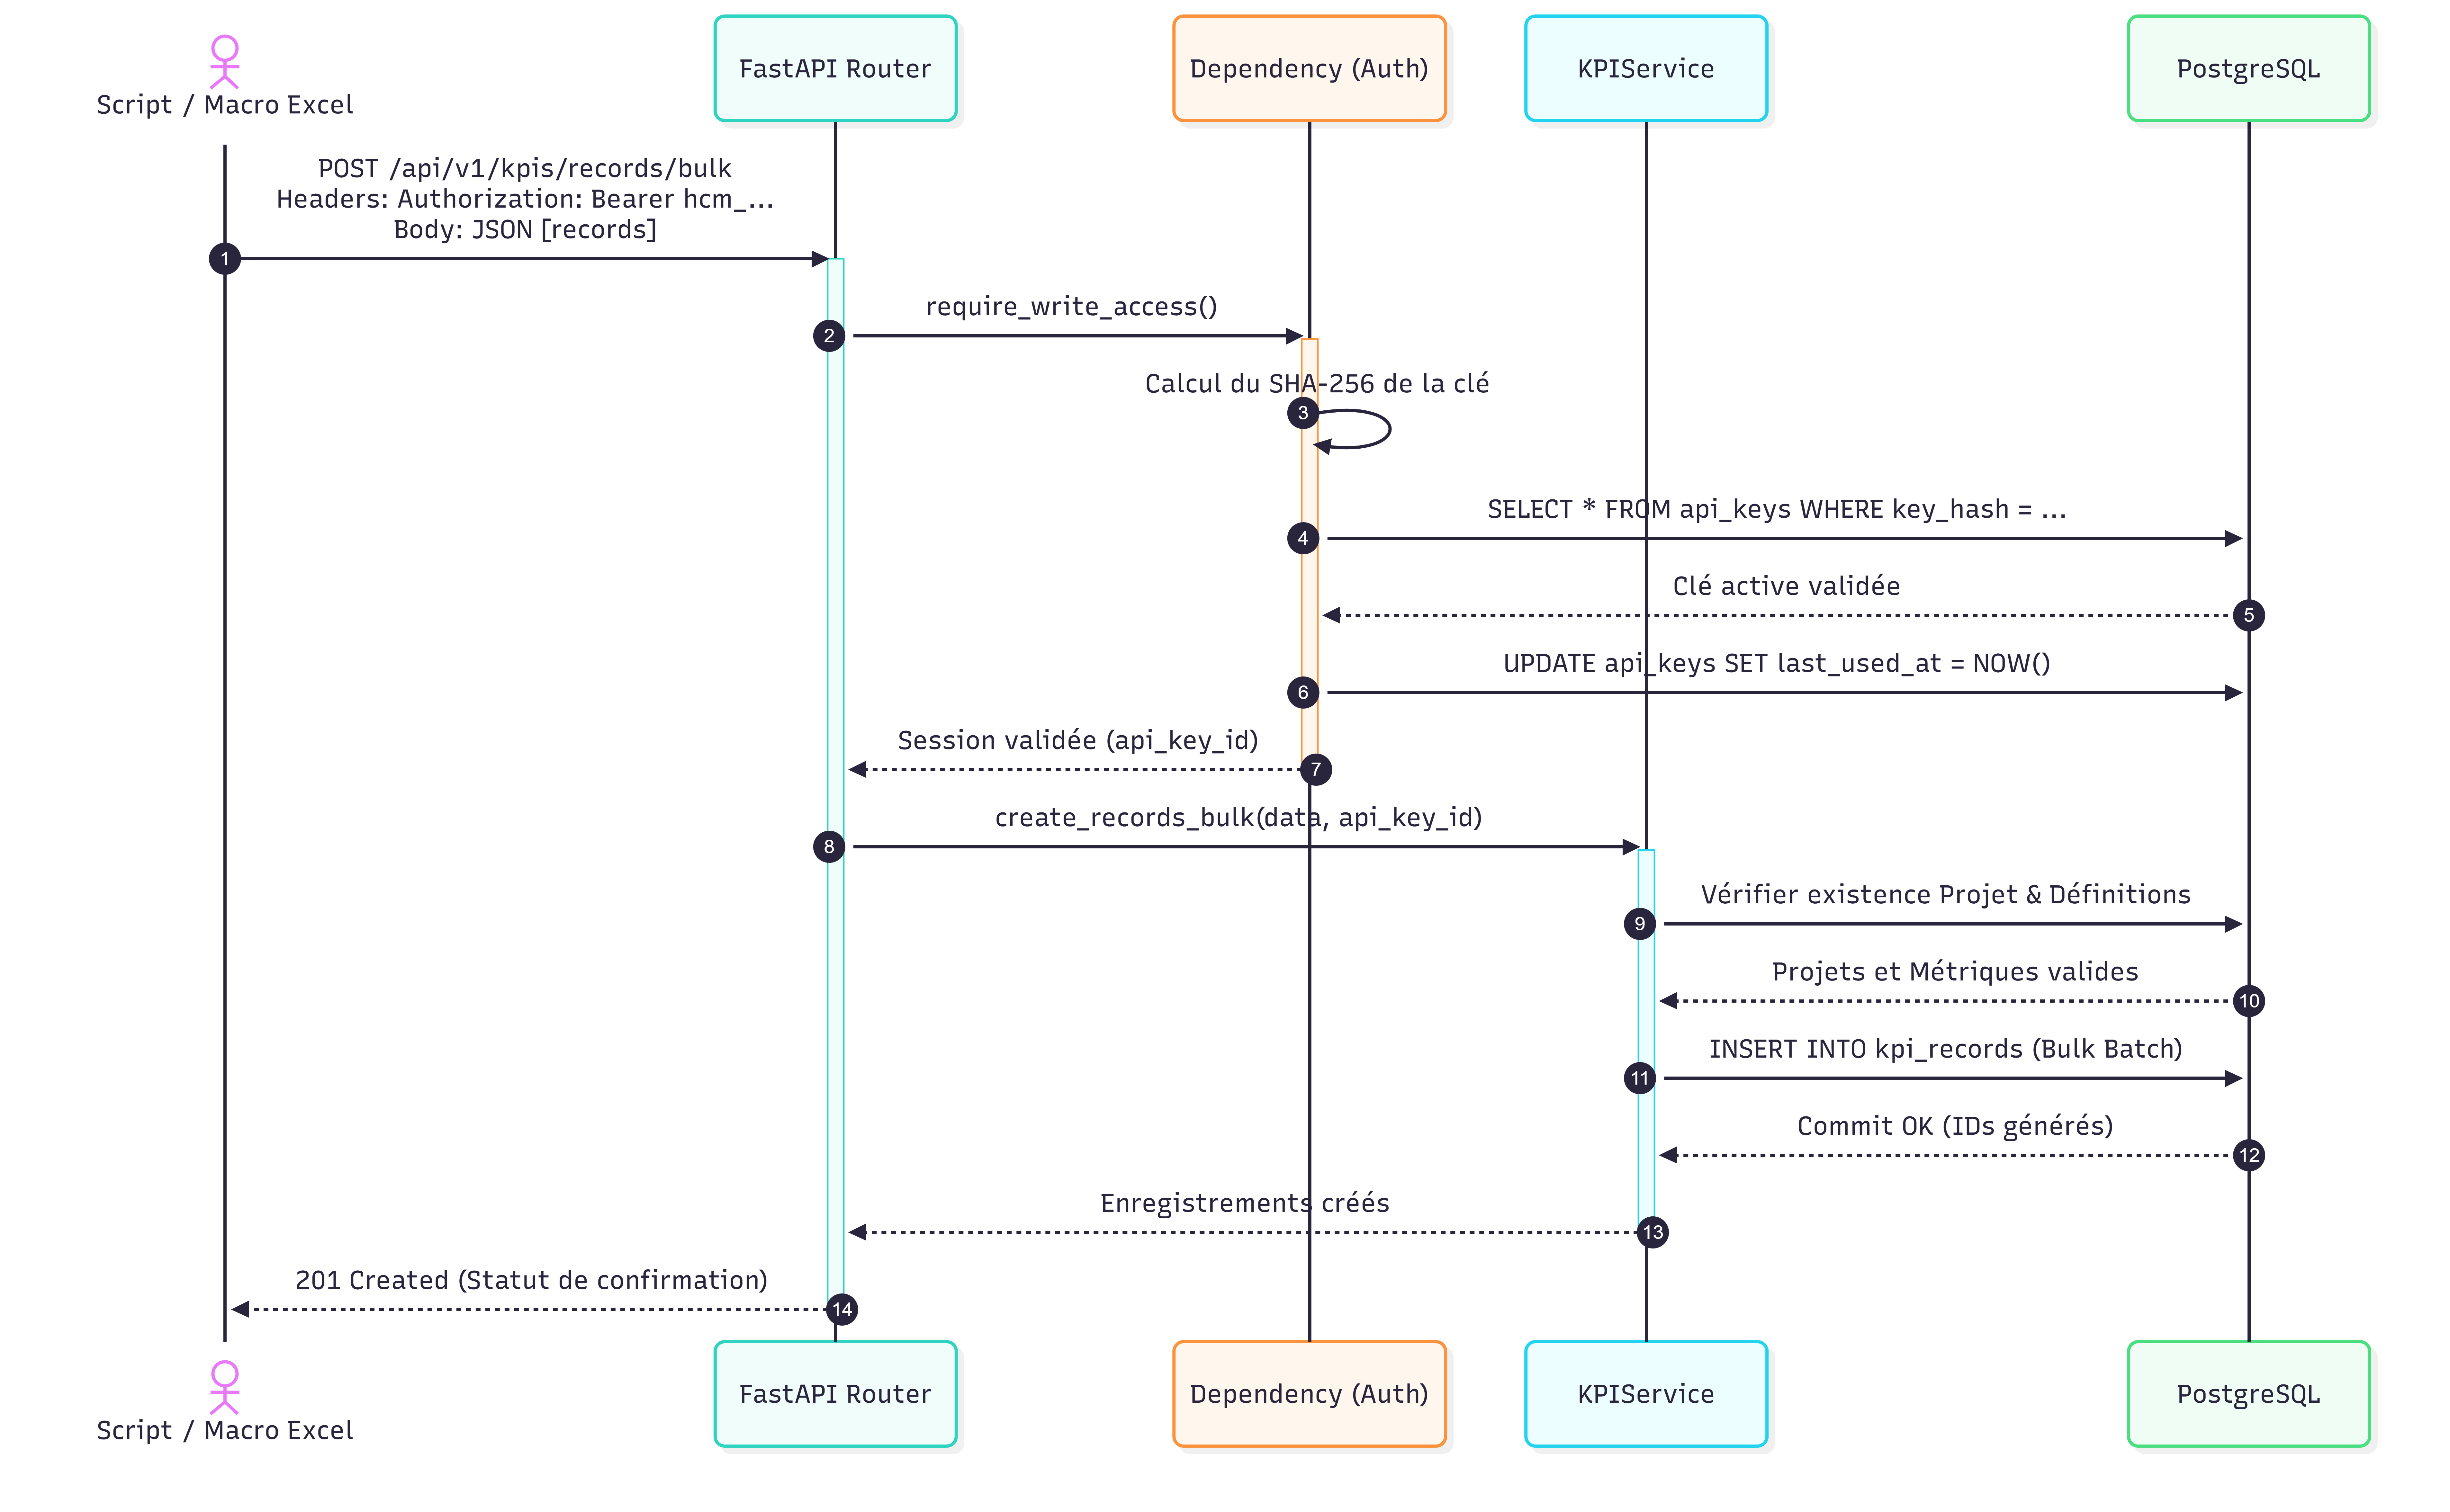
\includegraphics[width=0.85\textwidth]{images/ch4/sequence.png}
    \caption{Diagramme de séquence : Ingestion des données via API Key}
    \label{fig:seq_ingestion}
\end{figure}

\textbf{Description du flux :}
\begin{enumerate}
    \item Le script externe émet une requête \texttt{POST} contenant le payload JSON des KPIs, accompagnée de l'API Key dans l'en-tête \texttt{Authorization}.
    \item Le backend intercepte la requête, hache la clé et vérifie sa validité (statut actif, non expirée).
    \item Le service métier valide l'intégrité des données (existence du projet cible, types de valeurs).
    \item Les enregistrements sont insérés en lot (\textit{Bulk Insert}) de manière asynchrone dans PostgreSQL, et un code 201 (Created) est retourné.
\end{enumerate}

\subsection{Phase 2 : Restitution et Tableau de Bord}
Ce second flux illustre la récupération et la transformation des données lorsqu'un utilisateur (Manager) consulte le Dashboard.

\begin{figure}[H]
    \centering
    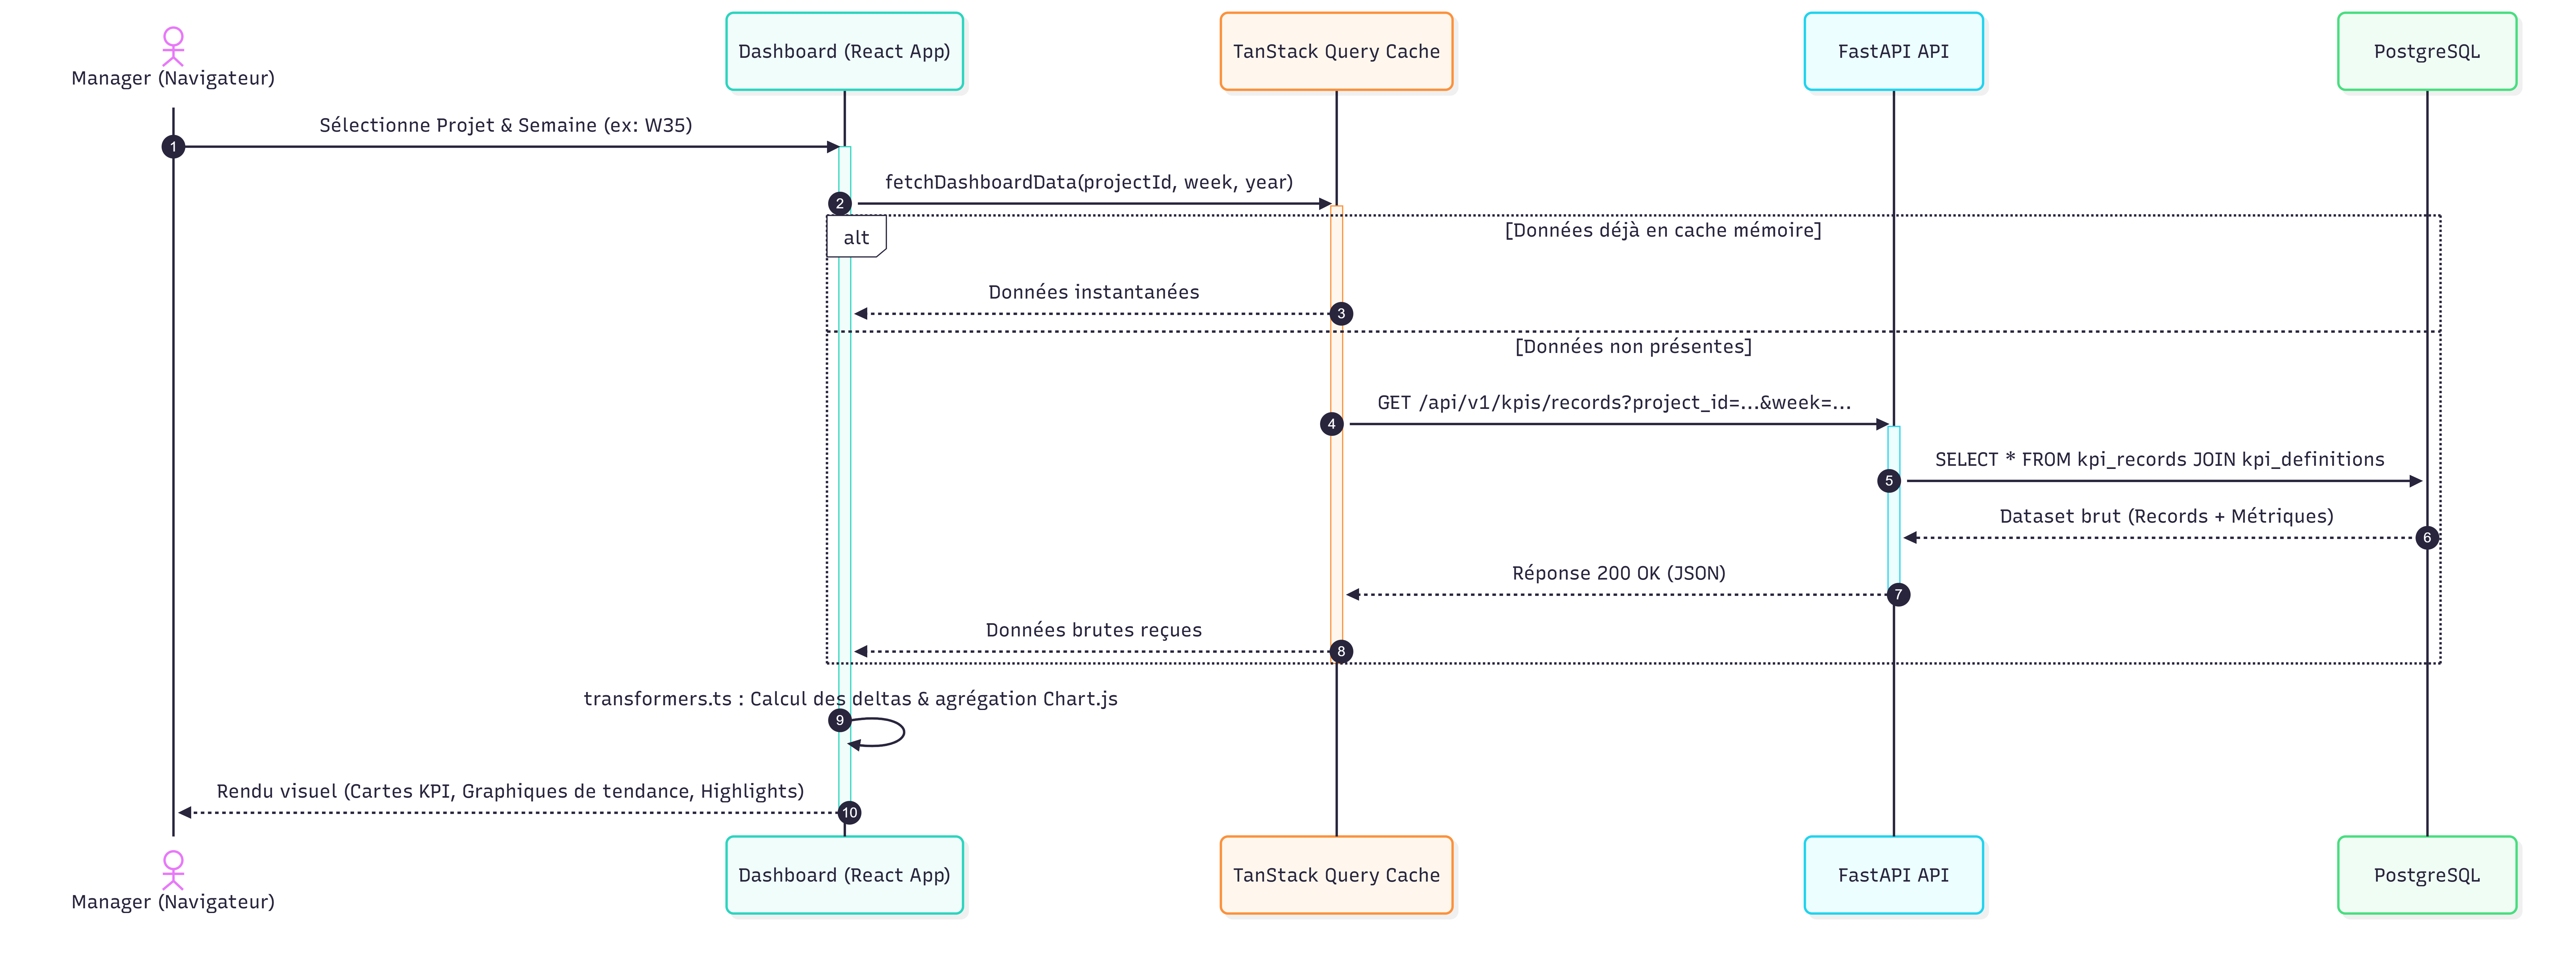
\includegraphics[width=0.85\textwidth]{images/ch4/seq_dashboard.png}
    \caption{Diagramme de séquence : Consultation du Dashboard}
    \label{fig:seq_dashboard}
\end{figure}

\textbf{Description du flux :}
\begin{enumerate}
    \item L'utilisateur sélectionne un projet et une période temporelle sur le Frontend.
    \item Le hook React (propulsé par TanStack Query) déclenche une requête \texttt{GET} vers le Backend.
    \item L'API interroge la base de données via l'ORM en effectuant une jointure optimisée entre les enregistrements (\texttt{KPIRecord}) et leurs définitions (\texttt{KPIDefinition}).
    \item Le Frontend reçoit le dataset brut. Un module de transformation côté client agrège les données, calcule les écarts différentiels (Deltas) et formate les séries chronologiques pour le rendu final dans les composants graphiques (\texttt{Chart.js}).
\end{enumerate}

\section*{Conclusion}
\addcontentsline{toc}{section}{Conclusion}
Les choix architecturaux et la modélisation retenus permettent de répondre efficacement aux problématiques identifiées. Le découplage des composants, associé à une modélisation robuste (Soft Delete) et une sécurité renforcée (Zero-Knowledge, JWT), assure la pérennité du système. Le chapitre suivant sera consacré à la réalisation concrète de cette architecture et à la présentation des interfaces finales.